% Provenance (never printed): see sources/outline_sources.md (Year 1: solute and particle
% fluxes; the Hjulstrom diagram; settling velocity; denudation rates). Exercise and problem
% values in the Book 3 scratch calculator calc/ch20.py; figure data from
% figdata/bachelor-1/settling.py and threshold.py. Erosion, transport and deposition are
% Book 1's (g5); the sediment load in three forms, the denudation rate and isostatic rebound
% are Book 2's (g12), re-founded here (load, denudation rate) or recalled (rebound); discharge
% and the drainage basin are Book 2 g10's; Airy isostasy is ch. 11's; viscosity, Stokes' law
% and the Reynolds number are the physics books' (admitted, pointer). Grain-size classes and
% sorting belong to ch. 21.
\chapter{Erosão e transporte}\label{ch:b1:erosion-transport}

Depois de uma tempestade, o rio sob a ponte corre barrento. A água que estava clara no dia anterior está grossa de lama, redemoinha em torno dos pilares e carrega galhos, e no leito, invisíveis, seixos se chocam uns contra os outros ao rolar. A cada segundo a enchente leva consigo toneladas de terra. Mais abaixo, atrás de uma represa, a mesma lama se deposita nas águas paradas do reservatório, que perde um pouco do seu volume a cada ano; mais longe ainda, na foz do rio, ela se espalha pelo mar como uma pluma marrom que pode ser vista do espaço. Este capítulo põe números nessa jornada: quanto um rio carrega e em que formas, quão depressa um grão afunda, que corrente é preciso para pô-lo em movimento, e quão depressa, no fim das contas, uma paisagem inteira é desgastada.

\begin{recall}
A erosão é o desgaste da terra e o transporte de seus fragmentos; a deposição é o depósito deles onde o transportador perde velocidade (Livro 1, 5º ano). Um rio transporta sua carga de sedimentos como \omterm{def:b1:erosion-transport:load}{carga de fundo}, \omterm{def:b1:erosion-transport:load}{carga em suspensão} e \omterm{def:b1:erosion-transport:load}{carga dissolvida}; a \omterm{def:b1:erosion-transport:denudation}{taxa de denudação} de uma região é a espessura de rocha dela removida por unidade de tempo, em metros por milhão de anos; quando a erosão remove uma espessura $e$ de \omterm{def:b1:layered-earth:layers}{crosta}, a recuperação isostática deixa a superfície descer apenas $e(1 - \rho_c/\rho_m)$ (Livro 2, 12º ano). A vazão de um rio é o volume de água que passa por uma seção transversal por unidade de tempo, e sua bacia de drenagem a área que o alimenta (Livro 2, 10º ano). Na \omterm{prop:b1:isostasy-gravity:airy}{isostasia de Airy} a \omterm{def:b1:layered-earth:layers}{crosta} flutua sobre o \omterm{def:b1:layered-earth:layers}{manto} com uma raiz proporcional a sua topografia (\cref{prop:b1:isostasy-gravity:airy}). A \omterm{def:b1:weathering-clays:hydrolysis}{hidrólise} dos silicatos envia íons e sílica dissolvida aos rios (\cref{def:b1:weathering-clays:hydrolysis}). A viscosidade dinâmica $\mu$ de um fluido mede sua resistência ao cisalhamento, e a viscosidade cinemática é $\nu = \mu/\rho$; uma esfera de diâmetro $d$ que se move lentamente à velocidade $w$ por um fluido sente o arrasto $3\pi\mu d w$ (lei de Stokes); o número de Reynolds $w d/\nu$ compara a inércia com as forças viscosas, e o escoamento em torno da esfera é suave enquanto ela for pequena (os livros de física).
\end{recall}

\section{Fluxos de soluto e de partículas}\label{sec:b1:erosion-transport:fluxes}

Um rio remove a terra de duas maneiras: como matéria em solução, os produtos do \omterm{def:b1:weathering-clays:weathering}{intemperismo químico}, e como grãos sólidos, os produtos do \omterm{def:b1:weathering-clays:weathering}{intemperismo físico} e os resíduos insolúveis do \omterm{def:b1:weathering-clays:weathering}{intemperismo químico}. As duas viajam de modos diferentes, e os próprios grãos viajam de dois modos.

\begin{definition}[Carga dissolvida, carga em suspensão, carga de fundo]\label{def:b1:erosion-transport:load}
A carga de um rio é a matéria que ele transporta além de uma seção transversal, em três partes que diferem pelo modo como viajam. A \emph{carga dissolvida}\index{carga dissolvida} é a matéria em solução, íons e sílica dissolvida, que se move com a água em sua própria velocidade. A \emph{carga em suspensão}\index{carga em suspensão} é formada por grãos mantidos no interior do escoamento pela sua turbulência, sobretudo argila, silte e areia fina, que se movem quase na velocidade da água e raramente tocam o leito. A \emph{carga de fundo}\index{carga de fundo} é formada por grãos que rolam, deslizam ou saltam ao longo do leito, em contato frequente com ele, muito mais devagar que a água.
\end{definition}

\begin{omfigure}
\begin{tikzpicture}[font=\footnotesize, >={Stealth[length=4pt]}]
% schematic: the three loads of a river (side view) and the forces on a bed grain
\fill[omDef!12] (0,0) rectangle (9,3.2);
\draw[omDef!80!black, thick] (0,3.2) -- (9,3.2);
\node[anchor=south west, omDef!80!black] at (0,3.2) {superfície da água};
% flow profile arrows (velocity grows upward)
\foreach \y/\l in {0.35/0.5, 0.8/0.9, 1.4/1.15, 2.1/1.3, 2.8/1.4} {\draw[->, black!55] (0.25,\y) -- ++(\l,0);}
\draw[black!55] (0.25,0.12) -- (0.25,3.05);
\node[anchor=north west, black!65, align=left] at (0.2,-0.15) {perfil de velocidade\\ do escoamento};
% bed
\fill[black!12] (0,-0.05) rectangle (9,0.12);
\foreach \x in {0.1,0.45,...,8.9} {\fill[black!45] (\x,0.0) circle[radius=0.09];}
% dissolved load: ions
\foreach \x/\y/\s in {2.3/2.7/+, 3.1/1.9/-, 4.0/2.85/+, 4.7/2.2/-, 5.6/2.75/+, 6.3/1.85/+, 7.2/2.6/-, 8.2/2.2/+, 2.7/1.2/-, 7.8/1.3/-} {\node[circle, draw=omThm, inner sep=0.2pt, minimum size=7pt, font=\tiny, text=omThm] at (\x,\y) {$\s$};}
% suspended load: fine grains, denser near the bed
\foreach \x/\y in {2.1/1.5, 2.6/0.9, 3.0/2.5, 3.4/0.6, 3.7/1.4, 4.2/0.8, 4.4/1.9, 4.9/0.55, 5.2/1.2, 5.5/2.1, 5.9/0.7, 6.1/1.5, 6.6/0.9, 6.9/2.3, 7.4/0.6, 7.6/1.7, 8.0/0.85, 8.5/1.4, 3.9/0.45, 5.0/0.35, 6.4/0.4, 2.4/0.45, 8.6/0.5} {\fill[brown!75!black] (\x,\y) circle[radius=0.05];}
% bed load: rolling and hopping grains
\fill[black!60] (3.2,0.27) circle[radius=0.15];
\draw[->, black!70] (3.0,0.55) arc[start angle=150, end angle=30, radius=0.25];
\fill[black!60] (5.6,0.25) circle[radius=0.12];
\draw[->, black!70, densely dashed] (4.6,0.2) .. controls (4.9,0.9) and (5.3,0.7) .. (5.55,0.4);
\fill[black!60] (4.6,0.22) circle[radius=0.06];
% labels
\node[omThm, anchor=west] at (9.2,2.5) {carga dissolvida: íons};
\node[brown!75!black, anchor=west] at (9.2,1.5) {carga em suspensão:};
\node[brown!75!black, anchor=west] at (9.2,1.1) {argila, silte, areia fina};
\node[black!75, anchor=west] at (9.2,0.4) {carga de fundo: rolando,};
\node[black!75, anchor=west] at (9.2,0.0) {deslizando, saltando};
\draw[->, thick, black!70] (6.8,3.55) -- node[above] {escoamento} (8.6,3.55);
% inset: forces on a grain resting on two others; it pivots about its downstream contact
\begin{scope}[xshift=11.8cm, yshift=-2.2cm]
  \fill[black!12] (-1.2,-0.4) rectangle (1.2,0);
  \fill[black!40] (-0.6,-0.15) circle[radius=0.28]; \fill[black!40] (0.6,-0.15) circle[radius=0.28];
  \fill[black!65] (0,0.166) circle[radius=0.4];
  \draw[->, thick, omDef!80!black] (0,0.166) -- (0,1.15) node[above] {sustentação};
  \draw[->, thick, omThm] (0,0.166) -- (1.05,0.166) node[right] {arrasto};
  \draw[->, thick, black] (0,0.166) -- (0,-0.8) node[below] {peso submerso};
  \draw[->, thick, black!60] (-1.4,0.85) -- (-0.5,0.85) node[pos=0, left] {escoamento};
  \fill[red!60!black] (0.353,-0.020) circle[radius=0.045];
  \node[font=\scriptsize, anchor=north west, black!70] at (0.5,-0.4) {pivô};
\end{scope}
\end{tikzpicture}

{\small As três cargas de um rio, vistas de lado (esquemático, fora de escala). O escoamento é mais rápido perto da superfície e se reduz a zero no leito. Íons se espalham por toda a profundidade; os grãos em suspensão são carregados pelos redemoinhos, mais deles perto do leito; os grãos da \omterm{def:b1:erosion-transport:load}{carga de fundo} rolam, deslizam ou dão pequenos saltos. À direita: as forças sobre um grão do leito. O arrasto e a sustentação do escoamento tendem a rolá-lo sobre seu vizinho de jusante, em torno do ponto de contato; seu peso na água o retém.}
\label{fig:b1:erosion-transport:loads}
\end{omfigure}

A fronteira entre as duas cargas sólidas não é fixada pelo tamanho do grão: depende do escoamento. Uma enchente que carrega areia em suspensão a deixa no leito, como \omterm{def:b1:erosion-transport:load}{carga de fundo}, quando baixa; a argila mais fina, por outro lado, permanece em suspensão em quase qualquer corrente e dificilmente é encontrada no leito de um rio que flui. Cada carga é medida como um fluxo, uma massa por unidade de tempo através de uma seção transversal do rio.

\begin{proposition}[Fluxo de uma carga]\label{prop:b1:erosion-transport:flux}
Seja $c$ a concentração de uma \omterm{def:b1:erosion-transport:load}{carga dissolvida} ou em suspensão (massa por unidade de volume de água) e $u$ a velocidade da água, ambas variando através da seção de área $A$. (1)~O fluxo instantâneo da carga através da seção é
\[
  F = \iint_A c\,u\,\mathrm dA = \overline{c}_Q\,Q,
\]
onde $Q = \iint_A u\,\mathrm dA$ é a vazão e $\overline{c}_Q$ a concentração média ponderada pela velocidade. (2)~Ao longo de um período $T$ em que a vazão $Q(t)$ e a concentração $C(t)$ do rio variam, a massa transportada é
\[
  M = \int_0^T Q\,C\,\mathrm dt = T\left(\overline{Q}\;\overline{C} +
  \operatorname{cov}(Q, C)\right),
\]
onde as barras são médias no tempo e $\operatorname{cov}(Q, C)$ é a média de $(Q - \overline{Q})(C - \overline{C})$. O produto da vazão média pela concentração média dá a massa correta apenas se as duas não forem correlacionadas.
\end{proposition}

\begin{proof}
(1)~Em um tempo $\mathrm dt$ a água que atravessa uma pequena área $\mathrm dA$ da seção preenche um volume $u\,\mathrm dA\,\mathrm dt$, que carrega a massa $c\,u\,\mathrm dA\,\mathrm dt$; somando sobre a seção dá $F$, e $\overline{c}_Q$ é definido como $F/Q$.
(2)~Escreva $Q = \overline{Q} + Q'$ e $C =
\overline{C} + C'$, em que as flutuações $Q'$ e $C'$ têm média nula ao longo do período. Então $QC = \overline{Q}\,\overline{C} + \overline{Q}\,C' + Q'\,\overline{C}
+ Q'C'$; os dois termos do meio têm média nula, e a média de $Q'C'$ é a covariância.
\end{proof}

A covariância importa para a \omterm{def:b1:erosion-transport:load}{carga em suspensão}. Sua concentração sobe abruptamente nas enchentes, quando a chuva lava o solo para os riachos e o escoamento mais rápido levanta grãos do leito, de modo que $Q$ e $C$ crescem juntos: uma grande parte do sedimento anual de um rio passa em poucos dias de enchente, e uma campanha de amostragem que as perca, ou uma concentração média multiplicada pela vazão média, subestima a carga. A \omterm{def:b1:erosion-transport:load}{carga dissolvida} se comporta ao contrário: as enchentes a diluem, e sua concentração é mais alta na vazão baixa, quando o rio é alimentado pela água subterrânea que esteve por muito tempo em contato com a rocha.

\begin{method}[A carga anual de um rio a partir de medições de vazão]\label{met:b1:erosion-transport:gauging}
\begin{enumerate}
  \item Registre a vazão continuamente em uma estação de medição.
  \item Amostre a água em muitas vazões, incluindo as enchentes, e meça a massa de sedimento por litro (por filtragem e pesagem) e de cada espécie dissolvida.
  \item Pondere as concentrações pela vazão no momento da amostragem para obter a concentração média ponderada pela vazão, ou ajuste a concentração como função da vazão e aplique-a a todo o registro.
  \item Multiplique pelo volume total de água do ano, ou some $Q\,C\,\Delta
        t$ sobre o registro (\cref{prop:b1:erosion-transport:flux}).
  \item Some a \omterm{def:b1:erosion-transport:load}{carga de fundo}, que os amostradores de água não captam, a partir de medições separadas ou como uma fração estimada.
  \item Para a \omterm{def:b1:erosion-transport:load}{carga dissolvida}, retire o que não vem da rocha: os sais trazidos pela chuva e, para o bicarbonato, o carbono retirado do ar (\cref{ch:b1:weathering-clays}).
\end{enumerate}
\end{method}

\begin{omfigure}
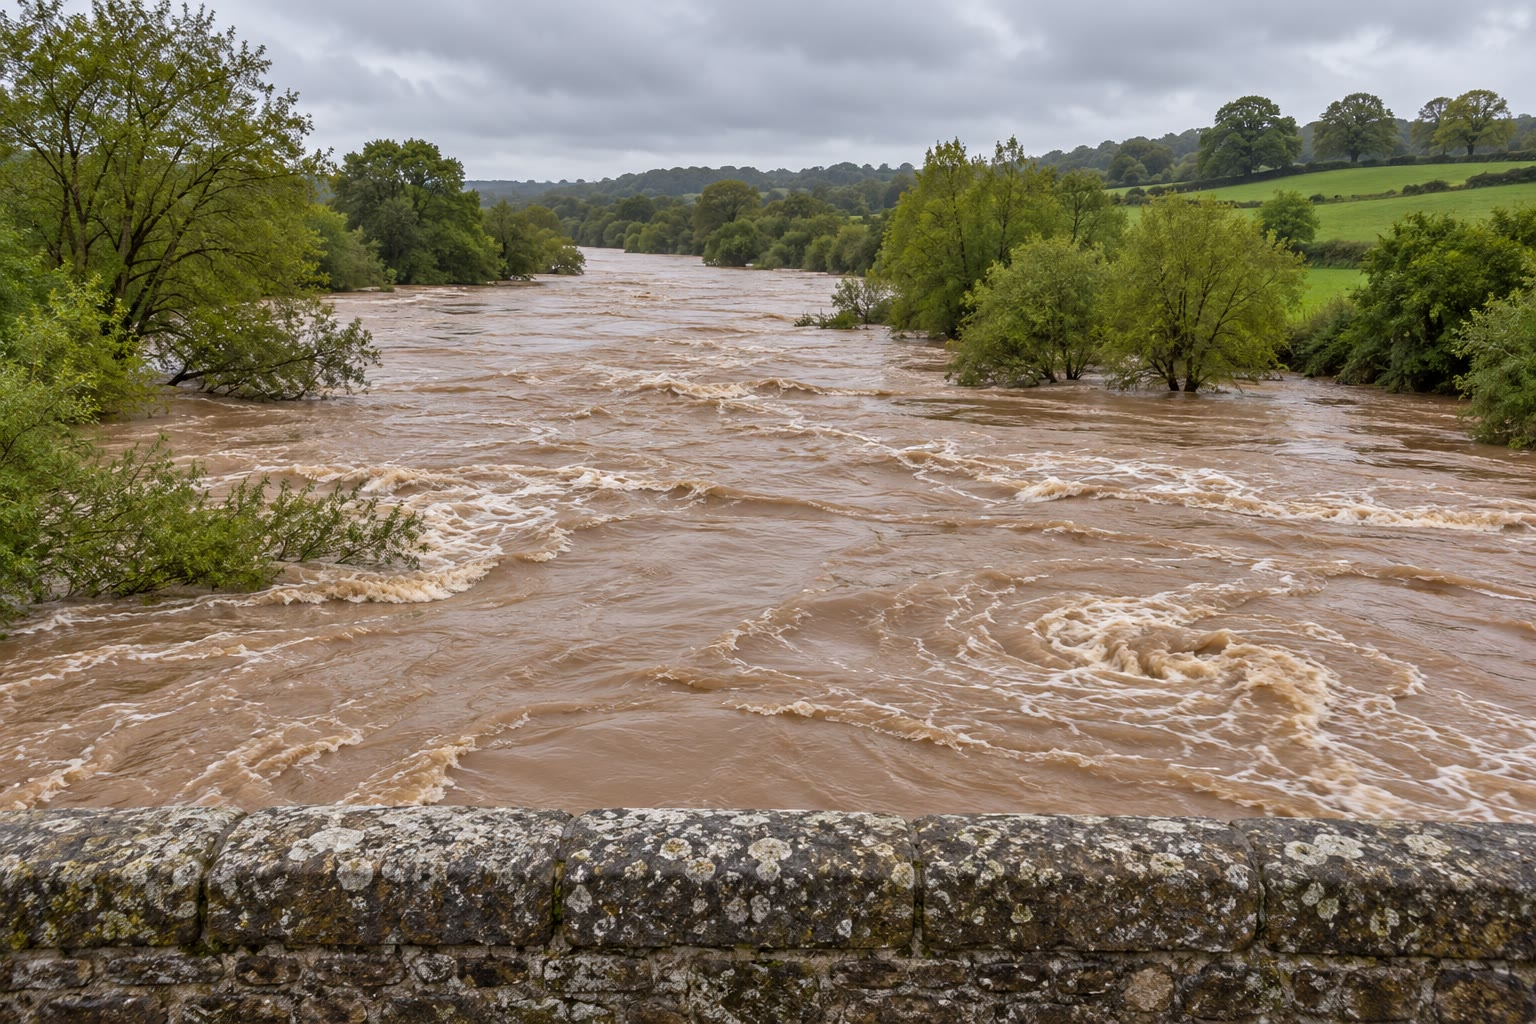
\includegraphics[height=5.1cm]{images/book3/ai/b1-muddy-river.jpg}\hfill
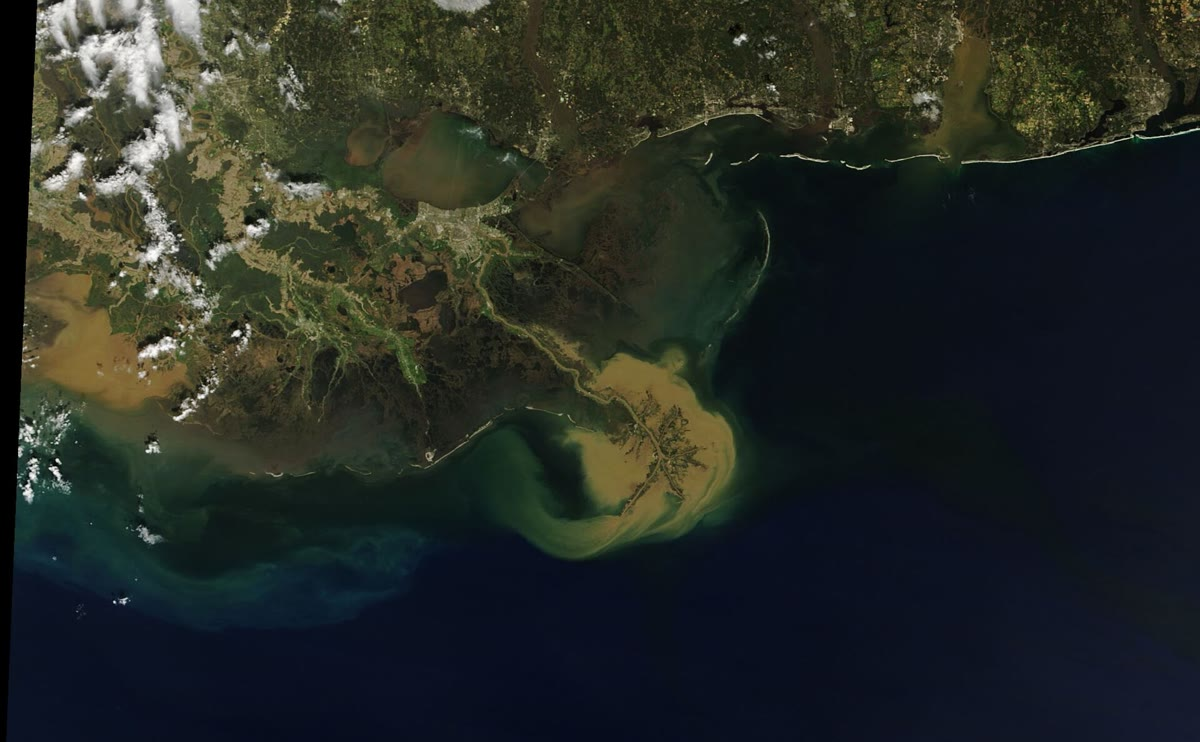
\includegraphics[height=5.1cm]{images/book3/b1-mississippi-plume.jpg}
{\small À esquerda: um rio em cheia carrega água marrom, carregada de sedimento (ilustração por IA). À direita: a pluma de cheia do Mississippi derramando-se no golfo do México em torno de seu delta, vista pelo instrumento MODIS no satélite Terra em 4~de março de 2018; a lama em suspensão colore o mar de marrom e verde, e o vento de sudeste empurra a pluma para noroeste. Imagem do Observatório da Terra da NASA, por Joshua Stevens, domínio público, via Wikimedia Commons.}
\label{fig:b1:erosion-transport:plume}
\end{omfigure}
% ledger: commons:mississippi-plume

\emph{Os rios do mundo.} Antes de qualquer influência humana, os rios do mundo levavam ao oceano costeiro uma estimativa de \qty{14}{Gt} de sedimento em suspensão por ano, \qty{15.5}{Gt} com a \omterm{def:b1:erosion-transport:load}{carga de fundo}. As pessoas mudaram as duas pontas da jornada: a agricultura e o desmatamento aumentaram a erosão do solo, somando cerca de \qty{2.3}{Gt} por ano aos rios, enquanto os reservatórios retêm sedimento: os grandes capturam cerca de \qty{20}{\percent} do fluxo e os pequenos mais \qty{6}{\percent}, e mais de \qty{100}{Gt} de sedimento jazem agora atrás de barragens construídas sobretudo nos últimos cinquenta anos. O efeito líquido é uma redução: o fluxo moderno é de cerca de \qty{12.6}{Gt} por ano.
% ledger: syvitski:flux

\begin{dated}{2005}
Os números do fluxo de sedimento em suspensão, antes e depois da influência humana, vêm de um modelo global de sedimento dos rios publicado em 2005. Barragens foram construídas desde então.
\end{dated}
% ledger: syvitski:flux

A \omterm{def:b1:erosion-transport:load}{carga dissolvida} é menor. Uma compilação clássica de análises de rios, feita em 1963, pôs a matéria dissolvida que os rios do mundo entregam ao mar em cerca de \qty{3.9}{Gt} por ano, cerca de \qty{30}{\percent} do fluxo moderno em suspensão, a uma concentração média de \qty{120}{mg} por litro. O bicarbonato forma quase a metade dela, \qty{58}{mg.L^{-1}}, seguido de cálcio, sílica, sulfato, cloreto e sódio. Parte dela não vem da rocha: boa parte do bicarbonato carrega carbono tirado do ar ou do solo, e parte do cloreto e do sódio vem de sal marinho trazido pela chuva. Rios individuais variam muito em torno dessas médias.
% ledger: livingstone:world-dissolved, syvitski:flux

\emph{O balanço de sedimentos de uma bacia.} Nem todo grão erodido em uma bacia de drenagem chega à sua saída. O solo lavado de um campo pode parar ao pé da encosta, a areia pode ser armazenada por séculos na planície de inundação e nos bancos do rio, e um reservatório pode reter a maior parte do que entra nele. A carga medida na saída é o saldo do balanço: o que é erodido nas encostas e nas margens, menos o que é armazenado no caminho, mais o que é retomado de depósitos antigos. Em algumas décadas de medição, esse saldo pode ficar bem distante da taxa de erosão de longo prazo, em qualquer direção, o que é uma das razões para os outros métodos de \cref{sec:b1:erosion-transport:denudation}.

\section{Velocidade de sedimentação}\label{sec:b1:erosion-transport:settling}

Um grão é mais denso que a água e afunda. Se um rio pode transportá-lo, e onde ele será depositado, depende antes de tudo da rapidez com que ele afunda.

\begin{definition}[Velocidade de sedimentação]\label{def:b1:erosion-transport:settling}
A \emph{velocidade de sedimentação}\index{velocidade de sedimentação} $w_s$ de um grão é a velocidade constante com que ele cai através de água parada, quando o arrasto da água equilibra seu peso submerso, seu peso menos o empuxo da água que ele desloca.
\end{definition}

Um grão liberado em água parada acelera até que seu arrasto, que cresce com sua velocidade, equilibre seu peso submerso; para um grão de areia ou silte isso leva uma pequena fração de segundo, de modo que a \omterm{def:b1:erosion-transport:settling}{velocidade de sedimentação} é a velocidade com que ele cai quase todo o trajeto. Com as densidades $\rho_s$ do grão e $\rho$ da água, escreva $R = (\rho_s - \rho)/\rho$ para a densidade submersa relativa.

\begin{proposition}[Sedimentação de Stokes]\label{prop:b1:erosion-transport:stokes}
Uma esfera de diâmetro $d$ e densidade $\rho_s$ caindo lentamente através de água de densidade $\rho$ e viscosidade dinâmica $\mu$, segundo a lei de Stokes, tem a \omterm{def:b1:erosion-transport:settling}{velocidade de sedimentação}
\[
  w_s = \frac{(\rho_s - \rho)\,g\,d^2}{18\,\mu} = \frac{R\,g\,d^2}{18\,\nu}.
\]
A lei vale enquanto o número de Reynolds do grão $w_s d/\nu$ estiver abaixo de cerca de 1, isto é, para diâmetros abaixo de $d_1 = \left(18\,\nu^2/(R\,g)\right)^{1/3}$.
\end{proposition}

\begin{proof}
O peso da esfera é $\rho_s g\,\pi d^3/6$ e o empuxo
$\rho g\,\pi d^3/6$, de modo que seu peso submerso é $(\rho_s - \rho)\,g\,\pi d^3/6$. Na \omterm{def:b1:erosion-transport:settling}{velocidade de sedimentação} ele se iguala ao arrasto $3\pi\mu d\,w_s$:
\[
  (\rho_s - \rho)\,g\,\frac{\pi d^3}{6} = 3\pi\mu d\,w_s
  \quad\Longrightarrow\quad
  w_s = \frac{(\rho_s - \rho)\,g\,d^2}{18\,\mu},
\]
e dividindo o numerador e o denominador por $\rho$ obtém-se a segunda forma. O número de Reynolds dessa velocidade é $R g d^3/(18\nu^2)$, que vale 1 para
$d = d_1$ e cresce como $d^3$.
\end{proof}

Para o quartzo, de densidade \qty{2650}{kg.m^{-3}}, em água a \qty{20}{\celsius},
de densidade \qty{998.2}{kg.m^{-3}} e viscosidade \qty{1.0016}{mPa.s}: $R =
1.65$, $\nu = \qty{1.003e-6}{m^2.s^{-1}}$, e com $g =
\qty{9.81}{m.s^{-2}}$ o limite é $d_1 = \qty{0.104}{mm}$, uma areia fina. Abaixo dele, a lei de Stokes dá as \omterm{def:b1:erosion-transport:settling}{velocidades de sedimentação} de silte e argila: um grão de silte de \qty{10}{\micro m} de diâmetro afunda a \qty{9.0e-5}{m.s^{-1}}, \qty{1}{m} em cerca de três horas; uma partícula de argila de \qty{2}{\micro m} a \qty{3.6e-6}{m.s^{-1}}, \qty{1}{m} em \num{3.2}~dias. As partículas naturais de argila são
placas, não esferas, e afundam ainda mais devagar. Água de \qty{5}{m} de profundidade, perfeitamente parada, levaria dezesseis dias para se clarear de tal argila; um rio em escoamento, cujos redemoinhos a mantêm agitada, nunca se clareia, e é por isso que a lama mais fina viaja até o mar.
% ledger: hom:quartz, nist:water, const:gn

Acima de $d_1$ o arrasto cresce mais que proporcionalmente à velocidade: a água que flui além do grão se separa atrás dele em uma esteira, e em números de Reynolds grandes o arrasto é proporcional ao quadrado da velocidade. Experimentos com grãos naturais são resumidos em uma única fórmula que une os dois regimes.

\begin{proposition}[Lei de sedimentação combinada]\label{prop:b1:erosion-transport:combined}
A \omterm{def:b1:erosion-transport:settling}{velocidade de sedimentação} de grãos naturais de diâmetro de peneira $d$ é, para todos os tamanhos,
\[
  w_s = \frac{R\,g\,d^2}{C_1\,\nu + \sqrt{0.75\,C_2\,R\,g\,d^3}},
\]
com $C_1 = 18$ e $C_2 = 1.0$.
\end{proposition}
\admitted
% ledger: fc:settling

A lei se deve a Ferguson e Church, que a ajustaram a \omterm{def:b1:erosion-transport:settling}{velocidades de sedimentação} medidas em areias naturais. Para grãos pequenos a raiz quadrada é desprezível e a lei se reduz à de Stokes; para grãos grandes o primeiro termo do denominador é desprezível e $w_s \to \sqrt{4 R g d/(3 C_2)}$, que cresce apenas como a raiz quadrada do tamanho. As constantes dependem da forma dos grãos: $C_2 = 0.4$ descreve esferas lisas, valores maiores, grãos mais angulosos, que encontram mais arrasto. As duas leis se separam acima de \qty{0.1}{mm}. Para um grão de \qty{1}{mm} a lei combinada dá \qty{0.126}{m.s^{-1}}, sete vezes menos que a de Stokes; para um seixo de \qty{10}{mm}, \qty{0.46}{m.s^{-1}} contra um absurdo \qty{90}{m.s^{-1}} (diagrama abaixo).
% ledger: fc:settling

\begin{omfigure}
\begin{tikzpicture}[font=\small]
% settling velocity of quartz grains in water at 20 C (figdata/bachelor-1/settling.py)
\begin{axis}[width=11cm, xmode=log, ymode=log, xmin=0.001, xmax=10, ymin=1e-8, ymax=10, height=8cm,
    xlabel={diâmetro do grão $d$ (\si{mm})}, ylabel={velocidade de sedimentação (\si{m.s^{-1}})},
    ytick={1e-8,1e-6,1e-4,1e-2,1},
    legend style={at={(0.03,0.97)}, anchor=north west, font=\footnotesize}, legend cell align=left,
    grid=major, grid style={black!10}]
  \addplot[omDef, thick, dashed] table[x=d_mm, y=w_stokes] {figdata/out/bachelor-1-settling-curves.dat};
  \addplot[omThm, very thick] table[x=d_mm, y=w_fc] {figdata/out/bachelor-1-settling-curves.dat};
  \legend{lei de Stokes, lei combinada (grãos naturais)}
  \draw[black!55, densely dotted] (axis cs:0.1037,1e-7) -- (axis cs:0.1037,10);
  \node[font=\scriptsize, anchor=west, align=left, black!75] at (axis cs:0.115,1e-6) {número de Reynolds\\ do grão $= 1$};
  \node[font=\scriptsize, black!70] at (axis cs:0.002,3e-8) {argila};
  \node[font=\scriptsize, black!70] at (axis cs:0.016,3e-8) {silte};
  \node[font=\scriptsize, black!70] at (axis cs:0.35,3e-8) {areia};
  \node[font=\scriptsize, black!70] at (axis cs:4.5,3e-8) {cascalho};
  \draw[black!40] (axis cs:0.0039,1e-8) -- (axis cs:0.0039,1e-7);
  \draw[black!40] (axis cs:0.0625,1e-8) -- (axis cs:0.0625,1e-7);
  \draw[black!40] (axis cs:2,1e-8) -- (axis cs:2,1e-7);
\end{axis}
\end{tikzpicture}

{\small \omterm{def:b1:erosion-transport:settling}{Velocidade de sedimentação} de grãos de quartzo em água a \qty{20}{\celsius} contra seu diâmetro, ambos em escalas logarítmicas: a lei de Stokes e a lei combinada de grãos naturais, calculadas. Nessas escalas a lei de Stokes é uma reta de inclinação 2. As duas concordam para silte e argila; acima de cerca de \qty{0.1}{mm}, onde o número de Reynolds do grão passa de 1, o arrasto da esteira freia os grãos grossos. As marcas na parte inferior assinalam as fronteiras das classes de tamanho de grão, em \qty{3.9}{\micro m} ($1/256$~mm), \qty{62.5}{\micro m} ($1/16$~mm) e \qty{2}{mm}.}
\label{fig:b1:erosion-transport:settling}
\end{omfigure}
% ledger: fc:settling, usgs:wentworth-phi

Ao longo da faixa do diagrama, da argila mais fina a um cascalho grosso, a \omterm{def:b1:erosion-transport:settling}{velocidade de sedimentação} abrange oito ordens de grandeza. Esta é a primeira razão pela qual os rios separam seus sedimentos: uma corrente que perde velocidade deposita de imediato o seu cascalho, sua areia a poucos metros, seu silte a poucos quilômetros, e leva sua argila a um lago ou ao mar. As classes de tamanho de grão e a seleção dos sedimentos são o assunto do próximo capítulo (\cref{ch:b1:clastic-sediments}).

\section{Limiar de movimento e o diagrama de Hjulström}\label{sec:b1:erosion-transport:threshold}

Um grão em repouso no leito de um rio é posto em movimento pela força da água que escoa sobre ele. Essa força é medida por uma tensão.

\begin{definition}[Tensão de cisalhamento no leito, velocidade de cisalhamento]\label{def:b1:erosion-transport:bed-shear}
A \emph{tensão de cisalhamento no leito}\index{tensão de cisalhamento no leito} $\tau_b$ de um escoamento é a força por unidade de área que ele exerce sobre seu leito, paralela ao leito, no sentido do escoamento. A velocidade de cisalhamento é $u_* = \sqrt{\tau_b/\rho}$, uma velocidade que mede a mesma tensão.
\end{definition}

A \omterm{def:b1:erosion-transport:bed-shear}{tensão de cisalhamento no leito} não pode ser lida em um medidor de corrente, mas em um escoamento permanente ela segue de um balanço de forças.

\begin{proposition}[Produto profundidade--declividade]\label{prop:b1:erosion-transport:depth-slope}
Em um escoamento permanente e uniforme de profundidade $h$ por um canal largo de pequena declividade $S$, a \omterm{def:b1:erosion-transport:bed-shear}{tensão de cisalhamento no leito} é
\[
  \tau_b = \rho\,g\,h\,S .
\]
\end{proposition}

\begin{proof}
Considere a água acima de um pedaço de leito de comprimento $L$ ao longo do escoamento e de largura unitária, sendo o canal tão largo que suas margens podem ser ignoradas. O escoamento é permanente e uniforme, de modo que essa água não acelera e as forças sobre ela se equilibram. As forças de pressão sobre suas faces de montante e de jusante são iguais e opostas, pois a profundidade é a mesma nas duas. Ao longo do escoamento restam a componente do peso, $\rho g h L \sin\beta$, em que $\beta$ é o ângulo do leito, e o atrito do leito, $\tau_b L$, a ela oposto. Logo $\tau_b
= \rho g h \sin\beta$, e para um ângulo pequeno $\sin\beta \approx \tan\beta = S$.
\end{proof}

Um rio de \qty{2}{m} de profundidade em uma declividade de \num{0.001}, um metro de queda por quilômetro, tem $\tau_b = 998.2 \times 9.81 \times 2 \times 0.001 =
\qty{19.6}{Pa}$, e uma velocidade de cisalhamento de \qty{0.140}{m.s^{-1}}. Em um canal que não é largo, as margens tomam sua parte do atrito, e a profundidade é substituída pelo raio hidráulico, a área da seção dividida por seu perímetro molhado (\cref{exo:b1:erosion-transport:5}).

\emph{Forças sobre um grão.} O escoamento empurra um grão do leito por seu arrasto e o levanta pela água mais rápida sobre seu topo (o detalhe da primeira figura deste capítulo). Ambas as forças atuam sobre a área do grão, de modo que escalam como $\tau_b
d^2$; o grão resiste por seu peso submerso, que escala como $(\rho_s - \rho) g d^3$. A razão entre as duas é a medida natural da intensidade do escoamento para um dado grão.

\begin{definition}[Parâmetro de Shields, limiar de movimento]\label{def:b1:erosion-transport:threshold}
O \emph{parâmetro de Shields}\index{parâmetro de Shields} de um escoamento de \omterm{def:b1:erosion-transport:bed-shear}{tensão de cisalhamento no leito} $\tau_b$ sobre grãos de diâmetro $d$ e densidade $\rho_s$ é
\[
  \theta = \frac{\tau_b}{(\rho_s - \rho)\,g\,d}.
\]
O \emph{limiar de movimento}\index{limiar de movimento} dos grãos é a \omterm{def:b1:erosion-transport:bed-shear}{tensão de cisalhamento no leito}, ou o valor $\theta_c$ do parâmetro de Shields, em que eles começam a se mover.
\end{definition}
% ledger: hecras:thresholds

O valor crítico $\theta_c$ é medido em canais de laboratório, e as medidas caem numa única curva quando plotadas contra um tamanho de grão adimensional que combina o grão e o fluido.

\begin{proposition}[Curva do limiar de Soulsby e Whitehouse]\label{prop:b1:erosion-transport:soulsby}
Para grãos de diâmetro $d$ sobre um leito plano, com
$D_* = d\,\left(R\,g/\nu^2\right)^{1/3}$, o \omterm{def:b1:erosion-transport:threshold}{parâmetro de Shields} crítico é
\[
  \theta_c = \frac{0.3}{1 + 1.2\,D_*} + 0.055\left(1 - e^{-0.02\,D_*}\right),
\]
e a tensão de cisalhamento crítica no leito é $\tau_c = \theta_c\,(\rho_s - \rho)\,g\,d$.
\end{proposition}
\admitted
% ledger: hecras:thresholds

Para grãos grossos $\theta_c$ tende a \num{0.055}: o cascalho se move quando a \omterm{def:b1:erosion-transport:bed-shear}{tensão de cisalhamento no leito} atinge cerca de um vigésimo do peso submerso de uma camada de grãos com um diâmetro de espessura, por unidade de área. As fórmulas de transporte de sedimentos que usam um limiar constante tomam valores de \num{0.03} a \num{0.047}, o último na clássica fórmula de \omterm{def:b1:erosion-transport:load}{carga de fundo} de Meyer-Peter e Müller. Para areia fina $\theta_c$ volta a crescer, para \num{0.077} a \qty{0.1}{mm}: grãos pequenos jazem dentro da camada lenta e viscosa de água junto ao leito e são abrigados por seus vizinhos. O mínimo, \num{0.030}, cai perto de \qty{0.7}{mm}. Em pascals o limiar sempre cresce com o tamanho (diagrama abaixo): \qty{0.13}{Pa} para uma areia de \qty{0.1}{mm}, \qty{0.51}{Pa} a \qty{1}{mm}, \qty{9.0}{Pa} a \qty{10}{mm}, \qty{57}{Pa} para um seixo de \qty{64}{mm}.
% ledger: hecras:thresholds

\begin{omfigure}
\begin{tikzpicture}[font=\small]
% threshold of motion of quartz grains in water at 20 C (figdata/bachelor-1/threshold.py, Soulsby and Whitehouse)
\begin{axis}[name=a, width=6.9cm, height=6cm, xmode=log, xmin=0.0625, xmax=100, ymin=0, ymax=0.12,
    xlabel={diâmetro do grão $d$ (\si{mm})}, ylabel={parâmetro de Shields crítico $\theta_c$},
    yticklabel style={/pgf/number format/fixed, /pgf/number format/precision=2},
    grid=major, grid style={black!10}, title={\footnotesize (a) adimensional}]
  \addplot[omThm, very thick] table[x=d_mm, y=theta] {figdata/out/bachelor-1-threshold-shields.dat};
  \draw[black!50, dashed] (axis cs:0.0625,0.055) -- (axis cs:100,0.055) node[pos=0.7, above, font=\scriptsize, black!70] {$0.055$};
\end{axis}
\begin{axis}[at={(a.east)}, anchor=west, xshift=2.0cm, width=6.9cm, height=6cm, xmode=log, ymode=log,
    xmin=0.0625, xmax=100, ymin=0.05, ymax=200,
    xlabel={diâmetro do grão $d$ (\si{mm})}, ylabel={tensão de cisalhamento crítica no leito $\tau_c$ (\si{Pa})},
    grid=major, grid style={black!10}, title={\footnotesize (b) em pascals}]
  \addplot[omDef, very thick] table[x=d_mm, y=tau_cr] {figdata/out/bachelor-1-threshold-shields.dat};
\end{axis}
\end{tikzpicture}

{\small O \omterm{def:b1:erosion-transport:threshold}{limiar de movimento} dos grãos de quartzo em água a
\qty{20}{\celsius}, a partir da curva de Soulsby e Whitehouse, calculado desde a fronteira da areia fina (\qty{0.0625}{mm}) até o tamanho de um seixo. (a)~O \omterm{def:b1:erosion-transport:threshold}{parâmetro de Shields} crítico é quase constante para cascalho e cresce para areia fina. (b)~A tensão de cisalhamento crítica no leito cresce quase em proporção ao diâmetro para o cascalho.}
\label{fig:b1:erosion-transport:threshold}
\end{omfigure}
% ledger: hecras:thresholds

\begin{example}[O que o rio move]\label{ex:b1:erosion-transport:river}
No rio de \qty{2}{m} de profundidade em declividade de \num{0.001}, $\tau_b =
\qty{19.6}{Pa}$. Para grãos de \qty{20}{mm}, $\theta = 19.6/(1651.8 \times
9.81 \times 0.020) = 0.060$, logo acima de seu limiar de \num{0.055}: eles se movem. Para grãos de \qty{40}{mm}, $\theta = 0.030$, metade do limiar: eles permanecem. O rio move seu leito até o cascalho grosso; para areia de \qty{1}{mm},
$\theta = 1.21$, quase quarenta vezes o limiar de \num{0.031}.
\end{example}

\emph{Em suspensão.} Uma vez em movimento, um grão salta ao longo do leito ou é arrastado para o escoamento, conforme os redemoinhos, cujas velocidades são da ordem da velocidade de cisalhamento, consigam sustentá-lo contra sua sedimentação.

\begin{proposition}[Critério de suspensão]\label{prop:b1:erosion-transport:suspension}
Um grão de \omterm{def:b1:erosion-transport:settling}{velocidade de sedimentação} $w_s$ pode permanecer em suspensão em um escoamento turbulento apenas se alguns redemoinhos subirem mais depressa do que ele afunda. Como as velocidades para cima dos redemoinhos são da ordem da velocidade de cisalhamento $u_*$, a suspensão começa quando $u_*$ se aproxima de $w_s$ e se desenvolve plenamente quando $u_*$ a excede; este capítulo toma $u_* = w_s$ como o limite da suspensão.
\end{proposition}
\admitted
% ledger: bagnold:suspension

No rio do exemplo, $u_* = \qty{0.140}{m.s^{-1}}$, que a lei combinada de sedimentação atribui a grãos de \qty{1.16}{mm}: areia mais fina que cerca de um milímetro viaja em suspensão, areia mais grossa e cascalho como \omterm{def:b1:erosion-transport:load}{carga de fundo}. O argumento remonta a Bagnold, que notou que grãos de \qty{0.1}{mm} ou menos ficam totalmente em suspensão assim que se movem, enquanto grãos maiores que \qty{1}{mm} precisam de uma \omterm{def:b1:erosion-transport:bed-shear}{tensão de cisalhamento no leito} muitas vezes acima de seu limiar. Quando a enchente baixa e $u_*$ cai, a areia grossa volta ao leito primeiro.

\emph{Da tensão à velocidade média.} O que é fácil de medir, ou de estimar, em um rio é sua velocidade média. Em um escoamento turbulento sobre um leito rugoso de grãos de diâmetro $d$, um canal largo de profundidade $h$ tem a velocidade média $U = u_*\left(6.25 + 5.75\log_{10}(h/d)\right)$, lei estabelecida por Keulegan em 1938 a partir dos experimentos de Nikuradse e Bazin; assim, o \omterm{def:b1:erosion-transport:threshold}{limiar de movimento} corresponde à velocidade média crítica
\[
  U_c = \left(6.25 + 5.75\,\log_{10}\frac{h}{d}\right)\sqrt{\theta_c\,R\,g\,d},
\]
e o limite de suspensão, $u_* = w_s$, a $U_s = \left(6.25 +
5.75\log_{10}(h/d)\right) w_s$. Ambas dependem da profundidade, embora só por meio de um logaritmo.
% ledger: keulegan:mean-velocity, bagnold:suspension

Velocidades de limiar pertencem, portanto, a uma profundidade e a um conjunto de leis: calculadas para outra profundidade, ou lidas de outras medidas, saem diferentes. Plotadas contra o tamanho do grão, sua forma é robusta, mas seus valores não, e a \omterm{def:b1:erosion-transport:bed-shear}{tensão de cisalhamento no leito}, que não depende da profundidade do mesmo modo, é a melhor medida do que um escoamento pode fazer. As velocidades são ainda as mais intuitivas, e a maneira clássica de desenhá-las é um diagrama.

\begin{definition}[Diagrama de Hjulström]\label{def:b1:erosion-transport:hjulstrom}
Um \emph{diagrama de Hjulström}\index{diagrama de Hjulström} representa a velocidade média de um escoamento contra o diâmetro dos grãos, em escalas logarítmicas, e divide o plano nos campos em que grãos em repouso são erodidos, grãos já em movimento são mantidos no transporte, e grãos em movimento são depositados.
\end{definition}
% ledger: hjulstrom:curve

\begin{omfigure}
\begin{tikzpicture}[font=\small]
% Hjulstrom-type diagram for a flow 1 m deep (figdata/bachelor-1/threshold.py); the hatched
% cohesive field is schematic (its lower edge, 30 cm/s, is not computed)
\begin{axis}[width=12cm, height=8.4cm, xmode=log, ymode=log, xmin=0.001, xmax=100, ymin=0.1, ymax=3000,
    xlabel={diâmetro do grão $d$ (\si{mm})}, ylabel={velocidade média do escoamento (\si{cm.s^{-1}})},
    unbounded coords=jump, grid=major, grid style={black!10}]
  \addplot[draw=none, name path=dep] table[x=d_mm, y=u_dep] {figdata/out/bachelor-1-threshold-hjul.dat};
  \addplot[draw=none, name path=bot] coordinates {(0.001,0.1) (100,0.1)};
  \addplot[fill=omDef!14, draw=none] fill between[of=dep and bot];
  \fill[pattern=north east lines, pattern color=omThm!45] (axis cs:0.001,30) rectangle (axis cs:0.0625,3000);
  \addplot[omThm, very thick] table[x=d_mm, y=u_cr] {figdata/out/bachelor-1-threshold-hjul.dat};
  \addplot[omDef, very thick, dashed] table[x=d_mm, y=u_s] {figdata/out/bachelor-1-threshold-hjul.dat};
  \node[font=\footnotesize, fill=white, fill opacity=0.85, text opacity=1, align=center] at (axis cs:0.5,1500) {\textbf{erosão}: grãos levados em suspensão};
  \node[font=\footnotesize, fill=white, fill opacity=0.85, text opacity=1, align=center] at (axis cs:22,330) {\textbf{carga de fundo}};
  \node[font=\footnotesize, fill=white, fill opacity=0.85, text opacity=1, align=center] at (axis cs:0.0042,2.5) {\textbf{transporte}:\\ grãos já em\\ movimento ficam\\ em suspensão};
  \node[font=\footnotesize, fill=white, fill opacity=0.85, text opacity=1, align=center] at (axis cs:3,0.6) {\textbf{deposição}};
  \node[font=\footnotesize, fill=white, fill opacity=0.85, text opacity=1, align=center] at (axis cs:0.008,300) {lama coesiva:\\ limiar fixado pela\\ compactação};
  \node[font=\scriptsize, omThm, anchor=north, rotate=12] at (axis cs:6,80) {limiar de movimento};
  \node[font=\scriptsize, omDef, anchor=north west, rotate=57] at (axis cs:0.028,0.95) {limite de suspensão};
  \draw (rel axis cs:0,0) -- (rel axis cs:1,0);
\end{axis}
\end{tikzpicture}

{\small Um diagrama do tipo Hjulström para grãos de quartzo em água de \qty{1}{m} de profundidade a \qty{20}{\celsius}, calculado: o \omterm{def:b1:erosion-transport:threshold}{limiar de movimento} (contínuo) a partir da curva de Soulsby e Whitehouse, o limite de suspensão (tracejado) a partir da lei de sedimentação combinada, ambos convertidos em velocidades médias pela lei de Keulegan. Acima da curva contínua, os grãos em repouso são erodidos; abaixo da mais baixa das duas curvas (sombreada), os grãos em movimento se depositam. Grãos mais finos que \qty{0.13}{mm} entram em suspensão assim que se movem; os mais grossos viajam primeiro como \omterm{def:b1:erosion-transport:load}{carga de fundo}. O cálculo vale apenas para grãos soltos: o campo hachurado de silte e argila coesos é esquemático.}
\label{fig:b1:erosion-transport:hjulstrom}
\end{omfigure}
% ledger: hecras:thresholds, fc:settling, bagnold:suspension, keulegan:mean-velocity

\emph{Lendo o diagrama.} Três traços carregam a geologia. Primeiro, os grãos mais fáceis de erodir são as areias finas, entre cerca de \num{0.06} e \qty{0.2}{mm}, que uma corrente de \qtyrange{31}{34}{cm.s^{-1}} põe em movimento em água de \qty{1}{m} de profundidade; grãos mais grossos precisam de mais, até cerca de \qty{3}{m.s^{-1}} para um seixo de \qty{64}{mm}. Segundo, silte e argila, embora mais leves, são mais difíceis de erodir que areia fina depois de assentados: suas partículas se grudam, e uma lama compactada resiste a uma corrente que levaria a areia embora. O cálculo para grãos soltos não consegue ver isso, e as velocidades de erosão medidas de lamas variam com sua compactação e teor de água, daí o campo hachurado. Terceiro, a lacuna entre erosão e deposição se abre bastante para os grãos finos: uma partícula de argila precisa de uma corrente forte para ser arrancada de um leito lamoso, mas, uma vez na água, permanece ali no escoamento mais brando, e essa é toda a história da enchente marrom e da pluma no mar.
% ledger: hjulstrom:curve, hecras:thresholds, keulegan:mean-velocity

\begin{history}[Dois estudos dos anos 1930]
Em 1935, Filip Hjulström, do Instituto Geográfico de Uppsala, publicou um longo estudo do trabalho do rio Fyris, no centro da Suécia, que continha o diagrama que leva seu nome: velocidades de erosão e de deposição contra o tamanho do grão, em escalas logarítmicas. Diferentemente de curvas anteriores, sua curva de erosão tinha um mínimo, entre cerca de \num{0.1} e \qty{0.5}{mm}: areia fina solta é a mais fácil de erodir, enquanto areias mais grossas e cascalho, e também silte e argila, que se coesionam, precisam de correntes mais fortes. Um ano depois, em 1936, o engenheiro A.~Shields,
na tese que defendeu na Escola Técnica Superior de Berlim, traçou o \omterm{def:b1:erosion-transport:threshold}{limiar de movimento} como uma razão de forças, o parâmetro que hoje leva seu nome, contra um tamanho de grão adimensional. As velocidades de Hjulström ignoram a profundidade do escoamento; a abordagem adimensional de Shields não, e ela sustenta as fórmulas de limiar usadas hoje, como a que está por trás dos diagramas deste capítulo.
\end{history}
% ledger: hjulstrom:curve, shields:1936, hecras:thresholds

\section{Taxas de denudação}\label{sec:b1:erosion-transport:denudation}

As cargas de um rio, somadas sobre sua bacia, medem a rapidez com que a bacia está sendo desgastada.

\begin{definition}[Taxa de denudação]\label{def:b1:erosion-transport:denudation}
A \emph{taxa de denudação}\index{taxa de denudação} $D$ de uma região é a taxa média com que a remoção de matéria, como grãos sólidos e em solução, rebaixa sua superfície, expressa como a espessura equivalente de rocha fresca por unidade de tempo, em metros por milhão de anos (\unit{m/Myr}, o mesmo que milímetros por mil anos). A massa removida por unidade de área e de tempo, em toneladas por quilômetro quadrado e por ano, é a produção específica de sedimento.
\end{definition}

\begin{proposition}[Denudação a partir das cargas de rio]\label{prop:b1:erosion-transport:denudation}
Se uma bacia de área $A$ perde, por sua saída, as massas anuais $F_s$ de \omterm{def:b1:erosion-transport:load}{carga em suspensão}, $F_b$ de \omterm{def:b1:erosion-transport:load}{carga de fundo} e $F_d$ de \omterm{def:b1:erosion-transport:load}{carga dissolvida} derivadas de suas rochas, e se nada é armazenado pelo caminho, sua \omterm{def:b1:erosion-transport:denudation}{taxa de denudação} é
\[
  D = \frac{F_s + F_b + F_d}{\rho_r\,A},
\]
com $\rho_r$ a densidade da rocha fresca. Para $\rho_r =
\qty{2700}{kg.m^{-3}}$, uma produção específica de \qty{100}{t.km^{-2}.yr^{-1}} corresponde a \qty{37}{m/Myr}.
\end{proposition}

\begin{proof}
A massa perdida por unidade de área e de tempo é $(F_s + F_b + F_d)/A$; dividida pela densidade da rocha, torna-se a espessura de rocha perdida por unidade de tempo. Para a conversão, \qty{100}{t.km^{-2}.yr^{-1}} é
$\qty{1e5}{kg}/\qty{1e6}{m^2} = \qty{0.1}{kg.m^{-2}}$ por ano, ou
$0.1/2700 = \qty{3.7e-5}{m}$ por ano, \qty{37}{m} por milhão de anos.
\end{proof}

A \omterm{def:b1:erosion-transport:load}{carga dissolvida} conta apenas a parte que vem da rocha, não a que vem do ar: o carbono do bicarbonato do intemperismo de silicatos é tirado da atmosfera, e só os cátions e a sílica são da rocha. A parte química da denudação não é pequena. Onde o clima é quente e úmido e a topografia baixa, ela pode se aproximar ou exceder a parte mecânica, enquanto em montanhas íngremes a parte mecânica domina.

\emph{Três relógios.} A \omterm{def:b1:erosion-transport:denudation}{taxa de denudação} pode ser medida em três escalas de tempo muito diferentes. As cargas de rios integram anos a décadas, e dependem das poucas enchentes que ocorreram, ou não, durante as medições. O sedimento retido em um reservatório ou em um lago, medido por levantamento de seu fundo, integra décadas a um século de sua vida. O terceiro relógio está escrito nos próprios grãos, pelos raios cósmicos.

\begin{proposition}[Nuclídeos cosmogênicos e erosão]\label{prop:b1:erosion-transport:cosmogenic}
Suponha que um nuclídeo seja produzido em uma rocha por raios cósmicos à taxa $P(z) = P_0\,e^{-\rho z/\Lambda}$ por unidade de massa, decrescendo exponencialmente com a profundidade $z$ ($\rho$ a densidade da rocha, $\Lambda$ uma constante, o comprimento de atenuação expresso como massa por unidade de área), e que a superfície desça à taxa constante $\varepsilon$. Desprezando o decaimento radioativo, um grão que atinge a superfície carrega a concentração
\[
  N = \frac{P_0\,\Lambda}{\rho\,\varepsilon}.
\]
\end{proposition}

\begin{proof}
Em relação à superfície, que desce à velocidade $\varepsilon$, um grão sobe à velocidade $\varepsilon$, de modo que passa o tempo $\mathrm dz/\varepsilon$ em uma camada de espessura $\mathrm dz$ à profundidade $z$, e ali ganha a concentração $P(z)\,\mathrm dz/\varepsilon$. Vindo de grande profundidade, atinge a superfície com
\[
  N = \frac{1}{\varepsilon}\int_0^{\infty} P_0\,e^{-\rho z/\Lambda}\,\mathrm dz
  = \frac{P_0}{\varepsilon}\,\frac{\Lambda}{\rho}. \qedhere
\]
\end{proof}

A concentração é inversamente proporcional à taxa de erosão: uma superfície que erode devagar mantém cada grão perto da superfície por muito tempo e o carrega de nuclídeos. A taxa que ela dá é média sobre o tempo necessário para erodir os poucos metros em que a produção se concentra, de cerca de mil a um milhão de anos, conforme a taxa. Desprezar o decaimento se justifica quando esse tempo é curto comparado com a vida do nuclídeo; quando a erosão é muito lenta, inclui-se o decaimento e a fórmula fica um pouco mais longa.
% ledger: portenga:method

\begin{inthelab}[Berílio-10 em areia de rio]
O nuclídeo usual é o berílio-10, de outro modo excepcionalmente raro na superfície da Terra, produzido por raios cósmicos no quartzo dos poucos metros superiores da rocha. Para medir a \omterm{def:b1:erosion-transport:denudation}{taxa de denudação} de uma bacia inteira, geoquímicos coletam areia do leito de seu rio perto da saída, na suposição de que o rio mistura grãos de cada encosta da bacia na proporção em que cada uma é erodida. No laboratório, o quartzo é separado dos outros \omterm{def:b1:rock-forming-minerals:mineral}{minerais} e limpo em ácidos que removem o berílio que o ar produziu e a chuva trouxe ao solo; em seguida
o quartzo é dissolvido, uma quantidade conhecida de berílio comum é adicionada, e o berílio é extraído. Seus isótopos são contados um átomo de cada vez com um espectrômetro de massa com acelerador, que consegue encontrar os raros átomos de berílio-10 entre um enorme excesso do isótopo comum.
\end{inthelab}
% ledger: portenga:method

\emph{Quais são as taxas.} Uma compilação de \num{1599} dessas medições, publicada em 2011, constatou que \omterm{def:b1:geological-maps:geological-map}{afloramentos} de rocha nua se rebaixam devagar: em \qty{12}{m/Myr} em média, com mediana de \qty{5.4}{m/Myr} (450 \omterm{def:b1:geological-maps:geological-map}{afloramentos}). A rocha sedimentar se desgasta mais depressa, \qty{20}{m/Myr} em média, que a metamórfica, \qty{11}{m/Myr}, e a ígnea, \qty{8.7}{m/Myr}. Bacias de drenagem inteiras perdem muito mais, \qty{218}{m/Myr} em média, com mediana de \qty{54}{m/Myr} (\num{1149} bacias): suas encostas íngremes, os deslizamentos e os canais dos rios se erodem muito mais depressa que seus cumes nus, e algumas bacias muito rápidas elevam a média quatro vezes acima da mediana. A declividade média de uma bacia é o melhor preditor único de sua taxa. Bacias em regiões sismicamente ativas, onde montanhas se erguem, têm média de \qty{367}{m/Myr}, contra \qty{182}{m/Myr} em regiões calmas; bacias polares, varridas por geleiras, \qty{537}{m/Myr}; bacias áridas, \qty{100}{m/Myr}.
% ledger: portenga:rates

\emph{A \omterm{def:b1:isostasy-gravity:isostasy}{isostasia} retarda o rebaixamento.} Retirar rocha de uma região em \omterm{def:b1:isostasy-gravity:isostasy}{isostasia} torna suas colunas mais leves, e a \omterm{def:b1:layered-earth:layers}{crosta} se eleva para restaurar o equilíbrio. Com $\rho_c
= \qty{2700}{kg.m^{-3}}$ e $\rho_m = \qty{3300}{kg.m^{-3}}$ (\cref{ch:b1:isostasy-gravity}), a fórmula de recuperação recordada no início do capítulo dá um rebaixamento de apenas $1 - 2700/3300 = 0.18$ da espessura removida: para baixar a superfície média de uma região em \qty{1}{m}, a erosão precisa remover \qty{5.5}{m} de rocha. O tempo para desgastar uma cordilheira é, assim, mais de cinco vezes o que sua altura dividida por sua \omterm{def:b1:erosion-transport:denudation}{taxa de denudação} sugere, e as rochas hoje na superfície de cordilheiras antigas e desgastadas já jaziam muitos quilômetros abaixo. E como a recuperação segue a espessura média removida, não sua distribuição, uma cordilheira cujos vales são cavados fundo enquanto seus picos mal são tocados se eleva como um todo: seus picos sobem, embora nada tenha sido acrescentado a eles (\cref{exo:b1:erosion-transport:11}).

\emph{As taxas mudam.} Uma \omterm{def:b1:erosion-transport:denudation}{taxa de denudação} medida hoje não é uma constante da paisagem. À medida que a topografia e as encostas diminuem, a taxa também diminui, e uma cordilheira antiga e rebaixada é desgastada cada vez mais devagar; inversamente, uma cordilheira que está sendo soerguida, ou um clima que muda, a eleva. Um tempo calculado a partir da taxa de hoje é uma primeira estimativa, não uma previsão.

\section{Exercícios}

\begin{exercise}[$\star$]\label{exo:b1:erosion-transport:1}
Um rio tem uma vazão média de \qty{500}{m^3.s^{-1}} e carrega, como média ponderada pela vazão, \qty{0.4}{g} de sedimento em suspensão por litro. Calcule seu fluxo em suspensão em quilogramas por segundo e em milhões de toneladas por ano (tome um ano de \num{365.25}~dias).
\end{exercise}

\begin{exercise}[$\star$]\label{exo:b1:erosion-transport:2}
Com a lei de Stokes, calcule a \omterm{def:b1:erosion-transport:settling}{velocidade de sedimentação} de um grão de silte de quartzo de \qty{30}{\micro m} de diâmetro em água a \qty{20}{\celsius} ($R = 1.6548$, $\nu =
\qty{1.0034e-6}{m^2.s^{-1}}$, $g = \qty{9.81}{m.s^{-2}}$), confira que seu número de Reynolds do grão é pequeno, e calcule o tempo que leva para afundar através de \qty{2}{m} de água parada.
% ledger: hom:quartz, nist:water
\end{exercise}

\begin{exercise}[$\star$]\label{exo:b1:erosion-transport:3}
Um riacho largo de \qty{0.5}{m} de profundidade escoa em declividade de \num{4e-4}. Calcule sua \omterm{def:b1:erosion-transport:bed-shear}{tensão de cisalhamento no leito}, com $\rho = \qty{998.2}{kg.m^{-3}}$, e o \omterm{def:b1:erosion-transport:threshold}{parâmetro de Shields} do escoamento para grãos de quartzo de \qty{1}{mm} e de \qty{10}{mm} ($\rho_s = \qty{2650}{kg.m^{-3}}$). Os valores críticos são \num{0.0314} a \qty{1}{mm} e \num{0.0556} a \qty{10}{mm}: quais grãos se movem?
% ledger: nist:water, hom:quartz, hecras:thresholds
\end{exercise}

\begin{exercise}[$\star$]\label{exo:b1:erosion-transport:4}
O fluxo moderno de sedimento em suspensão para o oceano é de cerca de \qty{12.6}{Gt} por ano, o fluxo dissolvido de cerca de \qty{3.9}{Gt} por ano, a uma concentração média de \qty{120}{mg.L^{-1}}. (a)~Qual é a razão entre o fluxo em suspensão e o dissolvido? (b)~Antes da influência humana o fluxo em suspensão era de \qty{14}{Gt} por ano: que massas os grandes reservatórios (\qty{20}{\percent}) e todos os reservatórios (\qty{26}{\percent}) retêm? (c)~Que volume anual de água fluvial o fluxo dissolvido e sua concentração implicam? Qual é então a concentração média de sedimento em suspensão, em gramas por litro?
% ledger: syvitski:flux, livingstone:world-dissolved
\end{exercise}

\begin{exercise}[$\star\star$]\label{exo:b1:erosion-transport:5}
Em um canal de largura finita, o produto profundidade--declividade torna-se $\tau_b =
\rho g R_h S$, com o raio hidráulico $R_h$, a área da seção dividida por seu perímetro molhado. (a)~Calcule $R_h$ para um canal retangular de \qty{10}{m} de largura e \qty{2}{m} de profundidade. (b)~Compare a \omterm{def:b1:erosion-transport:bed-shear}{tensão de cisalhamento no leito} em uma declividade de \num{0.001} com a de um canal muito largo da mesma profundidade. (c)~Mostre que $R_h \to h$ quando a largura cresce.
\end{exercise}

\begin{exercise}[$\star\star$]\label{exo:b1:erosion-transport:6}
(a)~Mostre a partir de \cref{prop:b1:erosion-transport:stokes} que o limite $d_1$ da lei de Stokes é proporcional a $\nu^{2/3}$. (b)~A \qty{10}{\celsius} a viscosidade da água é \qty{1.3059}{mPa.s} e sua densidade \qty{999.7}{kg.m^{-3}}; calcule $d_1$ para o quartzo, sabendo que ele é \qty{0.104}{mm} a \qty{20}{\celsius}, onde $\nu = \qty{1.0034e-6}{m^2.s^{-1}}$ (despreze a pequena mudança de $R$). (c)~De que fator um grão de silte de quartzo de \qty{50}{\micro m} afunda mais devagar a \qty{10}{\celsius} que a \qty{20}{\celsius}? O que isso significa para um rio no inverno?
% ledger: nist:water
\end{exercise}

\begin{exercise}[$\star\star$]\label{exo:b1:erosion-transport:7}
Para grãos de quartzo de \qty{0.1}{mm}, \qty{0.5}{mm} e \qty{2}{mm} em água a \qty{20}{\celsius}, calcule a \omterm{def:b1:erosion-transport:settling}{velocidade de sedimentação} pela lei de Stokes e pela lei combinada, e a razão entre as duas. Explique a tendência.
\end{exercise}

\begin{exercise}[$\star\star$]\label{exo:b1:erosion-transport:8}
(a)~Calcule, com a curva de Soulsby e Whitehouse, o \omterm{def:b1:erosion-transport:threshold}{parâmetro de Shields} crítico e a tensão de cisalhamento crítica no leito para grãos de quartzo de \qty{0.2}{mm} e
\qty{20}{mm}. (b)~Que profundidade de água, escoando permanentemente em um canal largo de declividade \num{0.002}, atinge cada limiar?
% ledger: hecras:thresholds
\end{exercise}

\begin{exercise}[$\star\star$]\label{exo:b1:erosion-transport:9}
Uma bacia de \qty{2000}{km^2} exporta por ano \qty{0.6}{Mt} de \omterm{def:b1:erosion-transport:load}{carga em suspensão} e de fundo e \qty{0.2}{Mt} de \omterm{def:b1:erosion-transport:load}{carga dissolvida} derivada da rocha. Calcule sua produção específica e sua \omterm{def:b1:erosion-transport:denudation}{taxa de denudação} para uma densidade da rocha de
\qty{2650}{kg.m^{-3}}. Como ela se compara com a mediana das bacias medidas com berílio-10?
% ledger: portenga:rates
\end{exercise}

\begin{exercise}[$\star\star\star$]\label{exo:b1:erosion-transport:10}
Um rio largo de \qty{3}{m} de profundidade escoa em declividade de \num{5e-4}. (a)~Calcule sua velocidade de cisalhamento e sua \omterm{def:b1:erosion-transport:bed-shear}{tensão de cisalhamento no leito}. (b)~Com
\cref{prop:b1:erosion-transport:suspension} e a lei combinada de sedimentação, encontre o maior grão de quartzo que ele carrega em suspensão. (c)~Com a curva de limiar, encontre o maior grão que ele move de todo. (d)~Descreva o leito e a carga deste rio.
% ledger: bagnold:suspension, hecras:thresholds, fc:settling
\end{exercise}

\begin{exercise}[$\star\star\star$]\label{exo:b1:erosion-transport:11}
Um platô em equilíbrio isostático é cortado por vales até que \qty{30}{\percent} de seu volume acima dos fundos dos vales seja removido; antes do corte ele estava como uma superfície plana \qty{1000}{m} acima dos futuros fundos dos vales. Tome $\rho_c = \qty{2700}{kg.m^{-3}}$ e $\rho_m = \qty{3300}{kg.m^{-3}}$. (a)~Que espessura média de rocha é removida? (b)~Quanto a região se eleva por \omterm{def:b1:isostasy-gravity:isostasy}{isostasia}? (c)~Quanto a superfície média foi rebaixada? (d)~O que aconteceu com os cumes que não foram erodidos?
\end{exercise}

\begin{exercise}[$\star\star\star$]\label{exo:b1:erosion-transport:12}
Um reservatório de \qty{50e6}{m^3} recebe \qty{0.5}{Mt} de sedimento por ano e retém \qty{90}{\percent} dele. O depósito, úmido e solto, tem densidade aparente de \qty{1300}{kg.m^{-3}}. (a)~Que volume do reservatório ele preenche a cada ano, e que fração? (b)~Quanto tempo até que metade do reservatório esteja cheia nesse ritmo? (c)~Por que a perda de volume costuma desacelerar à medida que o reservatório envelhece?
\end{exercise}

\section{Problema: com que rapidez as Colinas de Varden estão sendo desgastadas?}

\begin{problem}[{Problema de fim de semana --- o rio das Colinas de Varden, de suas cargas até o tempo necessário para desgastar as colinas}]
\label{pb:b1:erosion-transport:1}
% values: calc/ch20.py; the river and its gauging are invented (of a realistic order)
O rio das Colinas de Varden drena uma bacia de \qty{80}{km^2} de granito, xisto e rochas sedimentares. Em sua saída, uma estação de medição registra uma vazão média de \qty{1.2}{m^3.s^{-1}}; ao longo de vários anos de amostragem, a concentração média ponderada pela vazão de sedimento em suspensão é \qty{150}{mg.L^{-1}}, e a da \omterm{def:b1:erosion-transport:load}{carga dissolvida} derivada das rochas, \qty{80}{mg.L^{-1}}. A \omterm{def:b1:erosion-transport:load}{carga de fundo} é estimada em \qty{10}{\percent} da \omterm{def:b1:erosion-transport:load}{carga em suspensão}. Tome um ano de \num{365.25}~dias, uma densidade da rocha de \qty{2700}{kg.m^{-3}}, grãos de quartzo de densidade \qty{2650}{kg.m^{-3}}, e água a \qty{20}{\celsius} ($R
= 1.6548$, $\nu = \qty{1.0034e-6}{m^2.s^{-1}}$, $g = \qty{9.81}{m.s^{-2}}$).
% ledger: hom:quartz, nist:water, syvitski:flux, livingstone:world-dissolved

\medskip
\noindent\textbf{Parte I --- As cargas.}
\begin{enumerate}
  \item Exprima a vazão média como um escoamento superficial, a profundidade de água espalhada sobre a bacia a cada ano, em milímetros.
  \item Calcule o fluxo anual de sedimento em suspensão, em toneladas.
  \item Calcule o fluxo anual de \omterm{def:b1:erosion-transport:load}{carga dissolvida} derivada da rocha.
  \item Calcule a \omterm{def:b1:erosion-transport:load}{carga de fundo} e a carga total.
  \item A concentração média no tempo de sedimento em suspensão é bem menor que \qty{150}{mg.L^{-1}}. Explique por quê, e qual das duas deve ser multiplicada pela vazão média.
  \item Qual parcela do total a \omterm{def:b1:erosion-transport:load}{carga dissolvida} representa? Compare com os rios do mundo, cujo fluxo dissolvido é de cerca de \qty{3.9}{Gt} e o fluxo em suspensão de \qty{12.6}{Gt} por ano.
\end{enumerate}

\medskip
\noindent\textbf{Parte II --- A taxa de denudação.}
\begin{enumerate}[resume]
  \item Calcule a produção específica de sedimento da bacia.
  \item Calcule sua \omterm{def:b1:erosion-transport:denudation}{taxa de denudação}, em metros por milhão de anos.
  \item Compare-a com a mediana das bacias medidas com berílio-10, \qty{54}{m/Myr}. A bacia é rápida ou lenta?
  \item Uma medição de berílio-10 de areia da saída dá uma taxa da mesma ordem. Que intervalos de tempo a medição de vazão e o berílio fazem a média, e por que podem diferir?
  \item Por que só a parte da \omterm{def:b1:erosion-transport:load}{carga dissolvida} derivada da rocha deve ser contada?
\end{enumerate}

\medskip
\noindent\textbf{Parte III --- Um reservatório.}
Uma barragem é planejada na saída, retendo um reservatório de \qty{1.5e6}{m^3} com profundidade média de \qty{8}{m}.
\begin{enumerate}[resume]
  \item Qual é o tempo médio de residência da água no reservatório, em dias?
  \item Quanto tempo leva um grão de areia de quartzo de \qty{0.1}{mm}, entrando pela superfície, para afundar até o fundo (lei combinada)?
  \item Mesma pergunta para um grão de silte de \qty{0.02}{mm}, com a lei de Stokes.
  \item Mesma pergunta para uma partícula de argila de \qty{1}{\micro m}. Ela é retida?
  \item Qual é o grão mais fino que afunda através de toda a profundidade dentro do tempo de residência?
  \item Suponha que a \omterm{def:b1:erosion-transport:load}{carga de fundo} e \qty{70}{\percent} da \omterm{def:b1:erosion-transport:load}{carga em suspensão} sejam retidas, sendo o resto argila mais fina, e que o depósito tenha densidade aparente de \qty{1300}{kg.m^{-3}}. Que volume ele preenche a cada ano, que fração do reservatório, e quanto tempo até que esteja meio cheio?
\end{enumerate}

\medskip
\noindent\textbf{Parte IV --- Desgastando as colinas.}
\begin{enumerate}[resume]
  \item À \omterm{def:b1:erosion-transport:denudation}{taxa de denudação} da questão~8, quanto tempo levaria para rebaixar as colinas em \qty{100}{m}, se nada mais acontecesse?
  \item Com $\rho_c = \qty{2700}{kg.m^{-3}}$ e $\rho_m =
        \qty{3300}{kg.m^{-3}}$, de que fração da espessura removida a superfície média é rebaixada, uma vez que a \omterm{def:b1:isostasy-gravity:isostasy}{isostasia} tenha se ajustado?
  \item Que espessura de rocha precisa ser removida para rebaixar a superfície média em \qty{100}{m}?
  \item Se a erosão se concentra nos vales, o que acontece com os cumes mais altos durante esse tempo?
  \item Por que a taxa de hoje dificilmente se manterá constante por milhões de anos, e em que direção ela mudará?
  \item Em milhões de anos, com três algarismos, quanto tempo leva, à taxa de hoje e com a recuperação isostática, para rebaixar as Colinas de Varden em \qty{100}{m}?
\end{enumerate}
\end{problem}
